\documentclass{article}

\usepackage{blindtext}
\usepackage{graphicx}
\usepackage{wrapfig}
\usepackage[skip=1ex]{caption}
\usepackage{subcaption}
\usepackage{mdframed}
\usepackage{amsmath}
\usepackage{amsfonts}
\usepackage{amssymb}
\usepackage{amstext}
\usepackage{cancel}
\usepackage{enumitem}
\usepackage[english]{babel}
\usepackage{helvet}
\usepackage{microtype}
\usepackage[pdftex]{hyperref}
\usepackage{float}
\usepackage{nicematrix}
\usepackage{xcolor}
\usepackage{tikz}
\usepackage{geometry}
\geometry{
    a4paper,
    left=2cm,
    right=2cm,
    top=1cm,
    bottom=1cm
}

\special{papersize=8.5in,11in}
\setlength{\pdfpageheight}{\paperheight}
\setlength{\pdfpagewidth}{\paperwidth}

% Macros

% Make inline frac bigger
\newcommand\ifrac[2]{{\displaystyle\frac{#1}{#2}}}

% Aliases
\def\wstar{\overset{*}{\rightharpoonup}}
\def\grad{\nabla}
\def\lap{\Delta}
\def\nt{\notag}
\def\dt{\partial_t}
\def\hal{\ifrac{1}{2}}
\def\ep{\varepsilon}
\def\cK{\mathcal{K}}
\def\cA{\mathcal{A}}
\def\cS{\mathcal{S}}
\def\cV{\mathcal{V}}
\def\cJ{\mathcal{J}}
\def\cH{\mathcal{H}}
\def\Q{\mathbb{Q}}
\def\R{\mathbb{R}}
\def\R{\mathbb{R}}
\def\C{\mathbb{C}}
\def\la{\langle}
\def\ra{\rangle}
\def\ll{\langle\langle}
\def\rr{\rangle\rangle}

% Custom operators
\DeclareMathOperator{\Err}{Err}
\DeclareMathOperator{\re}{Re}
\DeclareMathOperator{\im}{Im}
\DeclareMathOperator{\id}{id}
\DeclareMathOperator{\dom}{dom}
\DeclareMathOperator{\img}{im}
\DeclareMathOperator{\coker}{coker}





\begin{document}



\title{Written Assignment 6}

\author{Niraj Venkat}

\date{}

\maketitle

\vspace{.8cm}

This is a statement of the Helmholtz-Hodge Decomposition theorem adapted from:
\begin{itemize}
    \item \href{https://brickisland.net/DDGSpring2021/2021/03/18/book-recommendation-for-differential-forms/}{Manifolds, Tensor Analysis, and Applications}
    (Marsden et. al.)
    \item \href{https://dl.acm.org/doi/10.1145/2818143.2818167}{Vector Field Processing on Triangle Meshes}
    (de Goes et. al.)
\end{itemize}

\begin{mdframed}
    Let $M$ be a compact, boundaryless, oriented, Riemannian manifold and let $\omega \in \Omega^k(M)$.
    Then there is an $\alpha \in \Omega^{k-1}(M), \beta \in \Omega^{k+1}(M), \,\text{and}\, \gamma \in \Omega^k(M)$ such that
    $$\omega = d\alpha + \delta\beta + \gamma$$
    Furthermore, $\alpha, \,\beta \,\text{and}\, \gamma$ are mutually $L^2$ orthogonal
    and so are uniquely determined. That is,
    $$\Omega^k(M) = d\Omega^{k-1}(M) \oplus \delta\Omega^{k+1}(M) \oplus \cH^k$$
    where $\Omega^k$ is the vector space of differential $k$-forms, and $\cH^k \subseteq \Omega^k$ is the subspace of harmonic $k$-forms.
\end{mdframed}

Put simply, the notion of $L^2$ inner product of tangent vector fields provides a very natural linear splitting 
of the space of vector fields on a smooth manifold. In the case of surfaces, this splitting implies that a 
tangent vector field can be orthogonally decomposed into three pieces:
\begin{itemize}
    \item \emph{gradient} (curl-free): $\grad \cdot \alpha = 0$, where $\alpha$ is called scalar potential
    \item \emph{rotated gradient} (divergence-free): $\grad \times \beta = 0$ where $\star\beta$ is called vector potential
    \item \emph{harmonic} (both curl and divergence-free): $\lap \gamma = 0$, where the Laplacian on $k$-forms is
    $\lap := d\delta + \delta d$
\end{itemize}
We aim to prove this in the following exercises.


\vspace{1.8cm}
\boxed{\text{Exercise} \quad 1}\\\\


Suppose we have linear operator $A$, $u \in \dom(A)$ and $v \in \coker(A)$. By definition $\coker(A) := \img(A)^\perp$,
so this inner product should be zero:
$$\ll Au, v \rr = 0$$
By definition of the adjoint:
$$\ll u, A^*v \rr = 0$$
Because $u$ can be non-zero, we have $u \in \img(A^*)^\perp$ and $v \in \ker(A^*)$.\\
Therefore, cokernel of a linear operator is the same as the kernel of its adjoint: $\coker(A) = \ker(A^*)$


\pagebreak
\boxed{\text{Exercise} \quad 2}\\\\


I tweak the notation from the problem, the empty set $\emptyset$ means 0.\\
$B \circ A = \emptyset$ means applying map $A$ then $B$ gives $\emptyset$:
\begin{align}
    \img(A) = \ker(B)^\perp
\end{align}
The union of a vector space and its orthogonal complement gives the entire space:
\begin{align*}
    \ker(B) \cup \ker(B)^\perp &= V \\
    \ker(B)^\perp \cap \ker(B) &= \emptyset \tag*{applying $\perp$ on both sides} \\
    \img(A) \cap \ker(B)^\perp &= \emptyset \tag*{using (1)} \\
    \img(A) \cap (\img(B^*)^\perp)^\perp &= \emptyset \tag*{$\img(A)^\perp = \ker(A^*)$} \\
    \img(A) \cap \img(B^*) &= \emptyset \\
\end{align*}
We used the idempotent properties of the adjoint and orthogonal complement.%: $* \circ * = \id$, $\perp \circ \perp = \id$


\vspace{1.8cm}
\boxed{\text{Exercise} \quad 3}\\\\


Any vector $v \in V$ can be split into two components -- along the image and cokernel of a map.\\

Decompose $v$ in relation to a map $A$:
$$
    v = Au + v^\prime
$$

for some $u \in U$ and $v^\prime \in \coker(A) = \ker(A^*)$. Now decompose $v^\prime$ in relation to a map $B^*$:
\begin{align*}
    v^\prime &= B^*w + z \\
    \implies v &= Au + B^*w + z
\end{align*}

for some $w \in W$ and $z \in \coker(B^*) = \ker(B)$. \\

Furthermore,
\begin{align}
    A^*v^\prime = 0 = A^*B^*w + A^*z
\end{align}

Now $Au \in \img(A)$ and $B^*w \in \coker(A)$ are orthogonal so we can write:
\begin{align*}
    0 &= \ll Au, B^*w \rr \\
        &= \ll u, A^*B^*w \rr
\end{align*}

For arbitrary $u$, we have $A^*B^*w = 0$. \\

Going back to expression (2),
\begin{align*}
    \cancelto{0}{A^*B^*w} + A^*z = 0 \\
    \implies A^*z = 0
\end{align*}

This shows that $z \in \ker(A^*) = \coker(A) = \img(A)^\perp$, and we also saw that $z \in \ker(B)$.
\begin{align*}
    \therefore z &\in \ker(B) \setminus \img(A) \\
    Au &\in \img(A) \\
    B^*w &\in \img(B^*)
\end{align*}

$V$ is decomposed into three mutually orthogonal subspaces.


\pagebreak
\boxed{\text{Exercise} \quad 4}\\\\

Since $M$ has no boundary, $\partial M = \emptyset$. \\

Adopting the convention $\star \omega(X) = -\omega(\cJ X)$ for a simpler calculation.
For a $k$-form $\alpha$ and $(k+1)$-form $\beta$:

\begin{align*}
    \ll d\alpha, \beta \rr &= \int_M d\alpha \wedge \star\beta \\
        &= \int_M d(\alpha \wedge \beta) - (-1)^k \alpha \wedge d\star\beta \\
        &= \int_{\partial M} \alpha \wedge \beta - \int_M (-1)^k \alpha \wedge d\star\beta \\
        &= 0 + (-1)^{k+1} \int_M \alpha \wedge d\star\beta \tag*{$\partial M = \emptyset$} \\
        &= (-1)^{k+1} (-1)^{k(n-k)} \quad \int_M \alpha \wedge \star (\star d\star\beta) \tag*{$\star\star \omega= (-1)^{k(n-k)} \omega$ for $k$-form in $\R^n$} \\
        &= (-1)^{nk-k^2+k+1} \int_M \alpha \wedge \star \delta\beta \\
        &= \pm \ll \alpha, \delta\beta \rr \tag*{Exponent for $-1$ is even only for $n, k$ both odd} \\
\end{align*}

%  $d$ and codifferential $\delta$ are adjoint. \\
P.S., \href{https://math.stackexchange.com/a/2829916}{Here is a proof}, which is more extensive. Covers both conventions.
What I learned from the proof is that codifferential $\delta$ should be defined such that based on our convention,
it cancels out the sign making it the adjoint of exterior derivative $d$ without this ambiguity.
% Here is the definition, with our convention above:
% $$
%     \delta\omega = (-1)^{n(n-k)+1} \star d \star \omega
% $$


\vspace{1.8cm}
\boxed{\text{Exercise} \quad 5}\\\\


We know that $d$ and $\delta$ are adjoint. Because $d^2 = 0$:
$$
    \ll d\alpha, \delta\beta \rr = \ll dd\alpha, \beta \rr = 0
$$

Together $d\alpha$ and $\delta\beta$ span a subspace of $k$-forms. The direct sum of this subspace with its orthogonal complement
gets us the full vector space of differential $k$-forms. This orthogonal complement would have:
$$
    \ll d\gamma, d\gamma \rr = \ll \delta\gamma, \delta\gamma \rr = 0
$$
which implies both $d\gamma = 0$ and $\delta\gamma = 0$.


\vspace{1.8cm}
\boxed{\text{Exercise} \quad 6}\\\\


Recall the musical isomorphisms: $\sharp$ takes forms to vectors, $\flat$ takes vectors to forms.

\begin{align*}
    \delta \beta &= \star d\star\beta \\
        &= \star d\star\star\phi \tag*{$\beta = \star\phi$} \\
        &= \star d\phi \tag*{$\star\star = \id$ for $n=2,k=0$} \\
        &= (d\phi)^\perp \tag*{$\star$ is a $90^\circ$ rotation for $n=2,k=1$} \\
        &= (((d\phi)^\perp)^\sharp)^\flat \\
        &= (((d\phi)^\sharp)^\perp)^\flat \tag*{Rotation commutes} \\
        &= ((\grad \phi)^\perp)^\flat \tag*{$\grad \phi = (d\phi)^\sharp$}
\end{align*}
The codifferential of a 2-form looks like the gradient, rotated by 90 degrees in the counter clockwise direction.


\vspace{1.8cm}
\boxed{\text{Exercise} \quad 7}\\\\


We use the definition $\lap := d\delta + \delta d$ and assume $\lap \gamma = 0$.\\

Let us assume $d\alpha$ is a $k$-form:
\begin{align*}
    \ll \Delta \gamma, \delta \beta \rr &= \ll d \delta \gamma + \delta d \gamma, \delta \beta \rr \\
        &= \ll d \delta \gamma, \delta \beta \rr + \ll \delta d \gamma, \delta \beta \rr \\
        &= \ll d d \delta \gamma, \beta \rr + \ll d \gamma, \delta d \beta \rr \\
        &= \ll d \gamma, \delta d \beta \rr \\
        &= 0
\end{align*}

For this to be true we must have $\gamma$ is closed, ($d \gamma = 0$).\\

Now assume $\delta \beta$ is a $k$-form:
\begin{align*}
    \ll \Delta \gamma, d \alpha \rr &= \ll d \delta \gamma + \delta d \gamma, d \alpha \rr \\
        &= \ll d \delta \gamma, d \alpha \rr + \ll \delta d \gamma, d \alpha \rr \\
        &= \ll \delta \gamma, \delta d \alpha \rr + \ll d \gamma, d d \alpha \rr \\
        &= \ll \delta \gamma, \delta d \alpha \rr \\
        &= 0
\end{align*}

For this to be true we must have $\gamma$ is co-closed, ($\delta \gamma = 0$).\\

By both definitions, $\gamma$ is harmonic.


\vspace{1.8cm}
\boxed{\text{Exercise} \quad 8}\\\\


From previous exercises:
\begin{align*}
    \img(A) \cap \ker(A^*) &= \img(A) \cap \coker(A) \\
        &= \img(A) \cap \img(A)^\perp \\
        &= \emptyset
\end{align*}


\vspace{1.8cm}
\boxed{\text{Exercise} \quad 9}\\\\


Start with:
$$
    d\alpha + \delta\beta + \gamma = \omega
$$

Applying $\delta$:
\begin{align*}
    \delta d\alpha + \delta\delta\beta + \delta\gamma &= \delta\omega \\
    \delta d\alpha + 0 + 0 &= \delta\omega \\
    \delta d\alpha &= \delta\omega
\end{align*}

Applying $d$:
\begin{align*}
    dd\alpha + d\delta\beta + d\gamma &= d\omega \\
    0 + d\delta\beta + 0 &= d\omega \\
    d\delta\beta &= d\omega
\end{align*}

Because $\delta^2 = d^2 = 0$, we end up with a linear system of equations in $\alpha$ and $\beta$.
This gives us an algorithm for decomposing a vector field.


\vspace{1.8cm}
\boxed{\text{Exercise} \quad 10}\\\\


\begin{figure}[h]
    \centering
    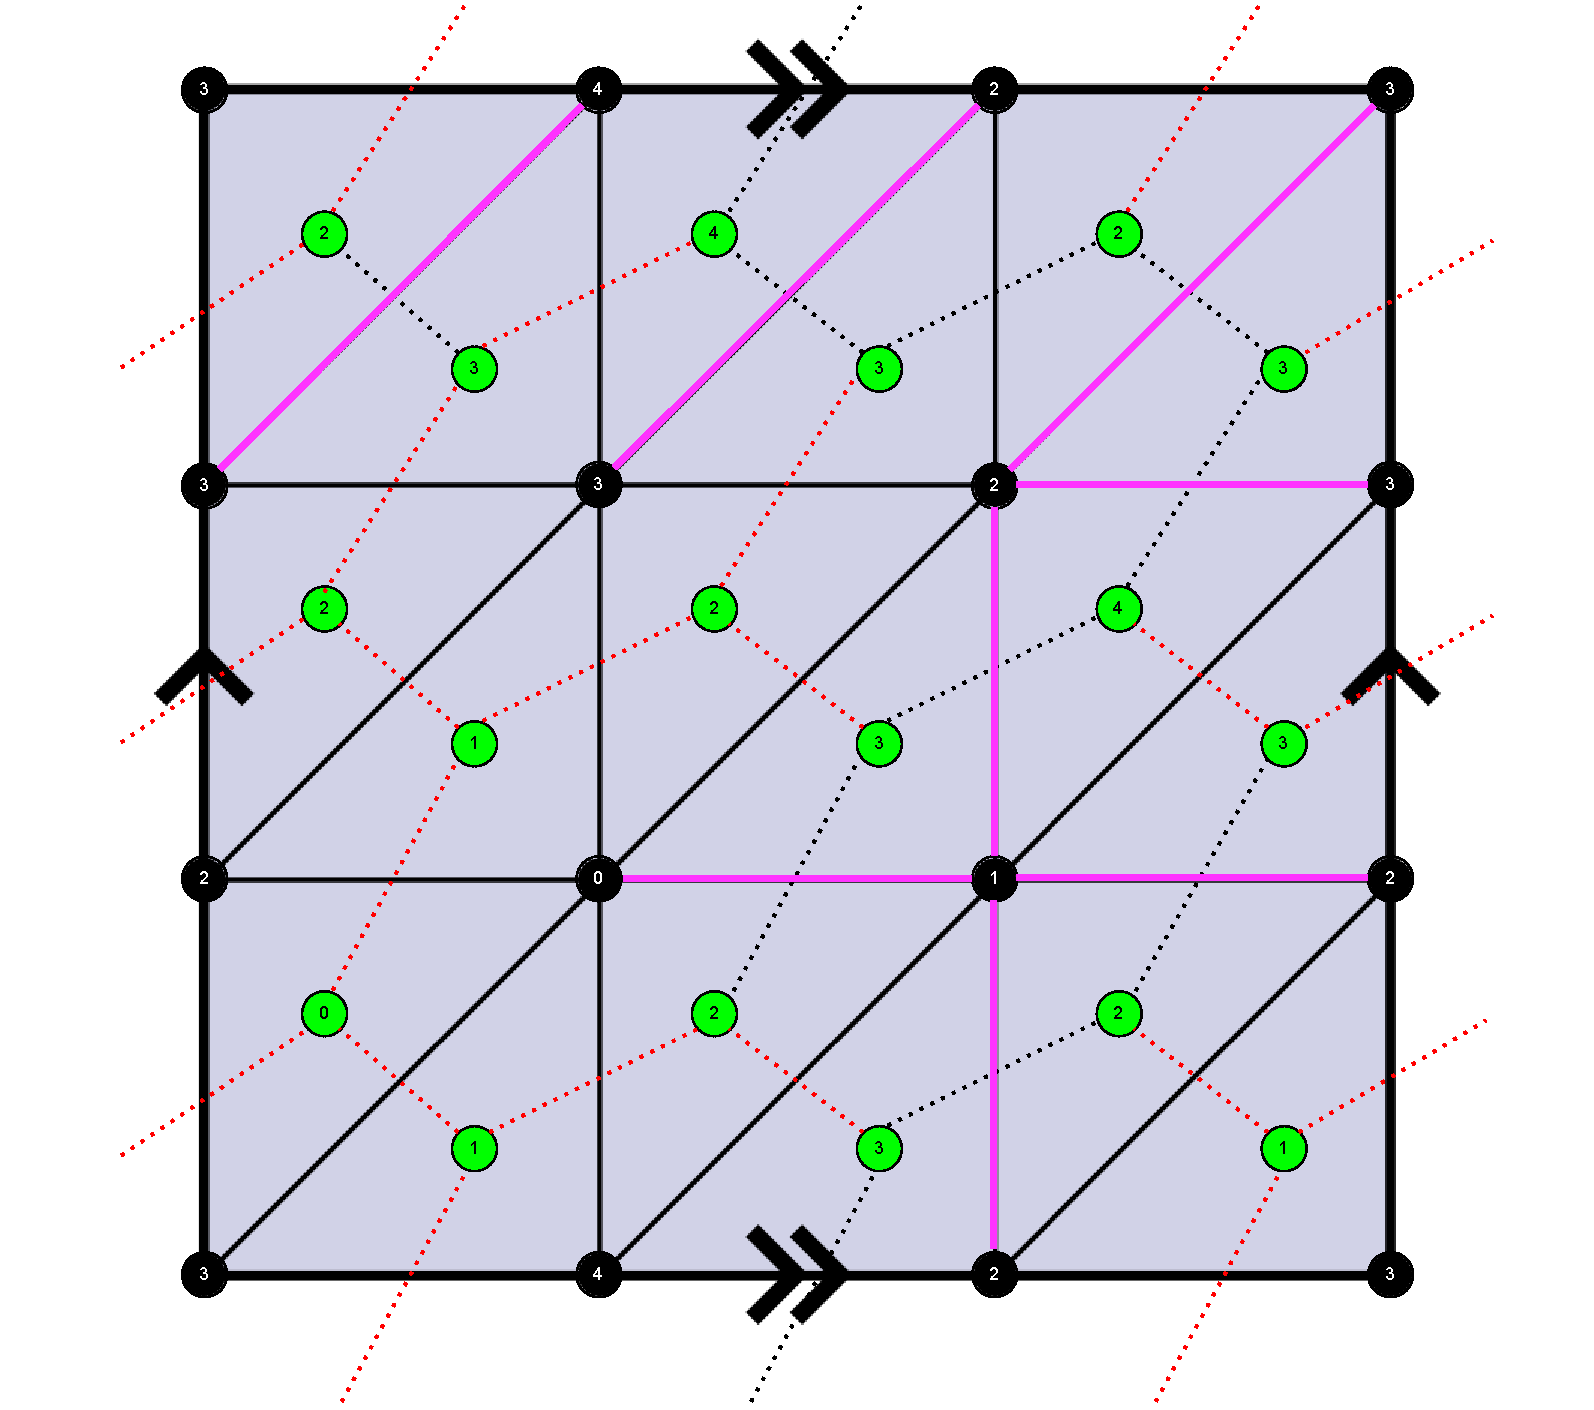
\includegraphics[width=\textwidth]{figs/torus_tree_cotree.pdf}
    \caption{Tree-Cotree for a torus}
\end{figure}

The Tree-Cotree algorithm is as follows:
\begin{enumerate}
    \item Build a spanning tree $T^*$ of dual edges
    \item Build a spanning tree $T$ of primal edges that do not cross edges in $T^*$
    \item For each dual edge $e^*_{ij}$ that is neither contained in $T^*$ nor crossed by $T$, follow both of its $ij$
        endpoints back to the root of $T^*$. The resulting loop is a generator.
\end{enumerate}

\vspace{0.8cm}

The dual graph has \textcolor{green}{green} vertices with dashed lines for edges. \textcolor{red}{Red} edges are in $T^*$, 
black edges are not.\\

The torus triangulation has black vertices with solid lines for edges. \textcolor{violet}{Violet} edges are in $T$, 
black edges are not. Identical vertices are identified, for example, the four corner vertices are actually the same vertex.\\

The number inside the vertex is the BFS traversal depth. $0$ is the root for the traversals in steps 1 \& 2.\\

Following step 3 gives us two loops (not shown here). We conclude that fundamental group $\pi_1(T^2)$ (first homology group) of a torus
has two generators, i.e, there are two equivalence classes of loops that can cannot be contracted to a point.\\

Torus has genus $g=1$ and matches the general prediction that a genus $g$ surface will have $2g$ generating loops for
its fundamental group.


\pagebreak
\boxed{\text{Exercise} \quad 11}\\\\

From the appendix of \href{http://geometry.caltech.edu/pubs/TACD06.pdf}{Designing Quadrangulations with Discrete Harmonic Forms}
by Tong et. al. and notes by \href{https://www.math.brown.edu/reschwar/M114/notes7.pdf}{Rich Schwartz}. \\

% Poincaré's lemma says that on a contractible manifold,
% like the sphere $S^2$, all closed forms are exact. 
% While $d^2=0$ implies that all exact forms are closed, it is not always true that all closed forms
% are exact.
We state the Poincaré Lemma:
\begin{mdframed}
    Let $M$ be an open star-shaped subset of $\R^n$ and let $\omega \in \Omega^r(M)$.
    Suppose that $d\omega = 0$. Then there is some $\alpha \in \Omega^{r-1}(M)$ such that $d\alpha = \omega$.
\end{mdframed}
A domain $M \subset \R^n$ is \emph{star-shaped} with respect to $p \in \R^n$ if, for each $q \in M$, the
entire segment $\overline{pq}$ lies in $M$. This applies to convex domains, but also piecewise flat domains like
the triangle mesh usually found in computational geometry. \\

In our problem we have a 1-form $\omega$ that is closed, i.e., $d\omega = 0$. If there is such a scalar potential (0-form)
$\alpha$ such that $d\alpha = \omega$ on the whole space, then $\omega$ is called exact. While $d^2=0$ 
implies that all exact forms are closed, it is not always true that all closed forms
are exact. In our case we can make no such guarantee on the existence of such a potential $\alpha$. \\

Taking the exterior derivative of both sides:
\begin{align*}
    0 &= d\omega \\
        &= d(d\alpha + \delta\beta + \gamma) \tag*{Helmholtz-Hodge Decomposition} \\
        &= dd\alpha + d\delta\beta + d\gamma \\
        &= d\delta\beta + d\gamma \tag*{$d^2 = 0$} \\
    \implies d\gamma &= -d\delta\beta \neq 0
\end{align*}

$\omega$ is not exact, it has a nonzero harmonic component. 


\vspace{1.8cm}
\boxed{\text{Exercise} \quad 12}\\\\


From the appendix of \href{https://www.cs.jhu.edu/~misha/ReadingSeminar/Papers/Gu03.pdf}{Global Conformal Surface Parameterization}
by Gu et. al.\\

A general surface $M$ can be represented as a sphere glued with several handles. Each handle has two special curves,
which when put together form a basis of the first homology group of $M$. When we cut $M$ along the homology basis, we get
a topological disk which has genus 0. The cohomology group is a linear functional space of the homology group.
In practice, we approximate smooth homology/cohomology with its simplicial variant. \\

Let $\ell_1, \dots , \ell_{2g}$ be a homology basis for our surface $M$ of genus $g$.
We can construct a corresponding 1-form $\omega_i$ for each loop $\ell_i$. Integrating $\omega$ over the boundary of 
an arbitrary simplex $\sigma$ and applying Stokes' theorem:
$$
    \int_{\partial\sigma} \omega = \int_\sigma d\omega = 0
$$
because $\omega$ is closed. \\

Any closed loop $r$ can be represented as a linear combination of $\ell_i$ with a patch boundary:
$$
    r = \sum_{i=1}^{2g} c_i \ell_i + \partial\sigma
$$

Applying Stokes' theorem again:
$$
    \int_r \omega = \sum_{i=1}^{2g} c_i \int_{\ell_i} \omega + \int_{\partial\sigma} \omega = 0
$$
Because $\int_{\ell_i} \omega = 0$, we find that integral of our closed 1-form $\omega$ over any closed loop $r$ is zero. \\

Earlier we showed that these linearly independent 1-forms have a harmonic component: $\omega_i = d\alpha_i + \gamma_i$. \\
Taking the inner product:
\begin{align*}
    \ll \gamma_i, \gamma_j \rr &= \ll \omega_i - d\alpha_i, \omega_j - d\alpha_j \rr \\
        &= 0
\end{align*}
Therefore each $\gamma_i$ is linearly independent and the space of harmonic 1-forms is $2g$ dimensional.


\vspace{1.8cm}
\boxed{\text{Exercise} \quad 13}\\\\


This is a physical experiment showcasing holonomy, and the action of the exponential map and the logarithmic map.\\

Basketball is our manifold $M$. Cardboard is the tangent space at a point $T_pM$.
Rolling without any twisting would be following a geodesic path, which is characterised by the exponential map:
$\text{exp}_p: T_pM \to M$.
If we twist as well, the connection 1-form $\omega: T_pM \to T_qM$ allows us to map between tangent spaces
at two distinct points $p, q$ on the manifold. Moreover, the Hopf-Rinow theorem tell us that if $M$ is a compact, 
connected Riemannian manifold, then any two points in $M$ are joined by a length minimizing geodesic. In other words,
$\omega$ is guaranteed to exist. \\

Following any connection, holonomy specifies the amount by which two tangent vectors fail to coincide after moving 
in a closed loop on surface $M$. Generally, holonomy is the difference in angle between an initial and final vector
that has been transported around a closed loop. In the case of the \emph{Levi-Civita connection}, holonomy
also happens to be the integrated Gaussian curvature over the region bounded by the closed loop.

\vspace{1.8cm}
\boxed{\text{Exercise} \quad 14}\\\\

For triangle meshes, the direction of parallel transport $Z$ is given by the dual edge $e^*_{ij}$
connecting two triangles that share an edge. A connection on a triangle mesh is described by a single angle $\phi_{ij}$
for each oriented dual edge in our mesh. In the discrete Levi-Civita connection all angles are zero. \\

Pullback of Gauss map would take tangent vectors on $S^2$ to tangent vectors on the surface $M$. `Unfold' step
in our procedure would be like collapsing the image of the Gauss map to a single point (making the entire surface have 
the same normal). `Translate' would keep the same normal as we travel across the the dual edge. `Refold' gets our original
Gauss map back, and we have also ensured that the two tangent spaces are the same.


\vspace{1.8cm}
\boxed{\text{Exercise} \quad 15}\\\\


Adapted from \href{https://www.cs.cmu.edu/~kmcrane/Projects/TrivialConnections/}{Trivial Connections on Discrete Surfaces}
by Crane et. al. \\

\begin{figure}[h]
    \centering
    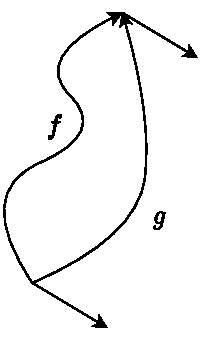
\includegraphics[scale=0.5]{figs/loop.pdf}
\end{figure}

A trivial connection guarantees that parallel transport is path-independent since any loop
$f \circ g^{-1}$ or $g \circ f^{-1}$ formed by combining paths $f$ and $g$ must have zero holonomy.
It does not matter if the loop is contractible or not. The only way the total change around the combined loop
can be zero is if change along $f$ equals the change along $g$.


\pagebreak
\boxed{\text{Exercise} \quad 16}\\\\


In a trivial connection, the adjustment angles (the difference between vectors in adjacent triangles) are computed
so that the connection can make any non-constant vector field a parallel one.


\vspace{1.8cm}
\boxed{\text{Exercise} \quad 17}\\\\


From Crane et. al. \\

A dual cell is a cycle of dual edges enclosing a vertex $v$. The angle defect $d(v)$ is simply the angle between
initial and final edges when these triangles are unfolded isometrically in the plane. More explicitly, given any initial
angle $\alpha_i$ in face $i$, we compute a new angle $\alpha_j$ in neighboring face $j$ as:
$$
    \alpha_j = \alpha_i - \theta_{ij} + \theta_{ji}
$$
where $\theta_{ij}$ and $\theta_{ji}$ are the angles between the shared edge $e$ and an arbitrary but fixed
reference direction in triangles $i$ and $j$, respectively. \\

Repeating this procedure for $n$ consecutive dual edges in a cycle gives us a sequence of angles
$\alpha_0, \dots, \alpha_n$, and the resulting angle defect is given by $d(v) = \alpha_n - \alpha_0$.
Earlier we learned that $d(v)$ is used to define a discrete notion of Gaussian curvature at a vertex.
This is the holonomy of the discrete Levi-Civita connection.


\vspace{1.8cm}
\boxed{\text{Exercise} \quad 18}\\\\


For a topological disk $D$, Euler number $\chi = 0$. \\
Earlier we showed that the sum of Gauss curvatures $K_v$ is the sum of angle defects $d(v)$. \\
From Gauss-Bonnet:
$$
    \sum_{v \in V} K_v  = \sum_{v \in V} d(v) = 2\pi\chi = 0
$$
Also the holonomy around boundary $\partial D$
is the curvature of the discrete Levi-Civita connection over region $D$, which equals zero.


\vspace{1.8cm}
\boxed{\text{Exercise} \quad 19}\\\\


We just showed that holonomy around any discrete loop is determined by the curvature of the connection.
Moreover, any loop on a genus $g$ surface can be built as a linear combination of a basis of $2g$ non-contractible loops,
or generators of the fundamental group.


\vspace{1.8cm}
\boxed{\text{Exercise} \quad 20}\\\\


We can change the constraint:
\begin{align*}
    d_0^T \phi &= -K + 2\pi k \\
    \implies d_0^T d_1^T d_1 \phi &= 0
\end{align*}   
because $d_1^T d_1 = \id$ and $d_0^T d_1^T = 0$. So the null space of $d_0^T$ is spanned by the columns of $d_1^T$.


\vspace{1.8cm}
\boxed{\text{Exercise} \quad 21}\\\\


Taken from \href{https://www.cs.cmu.edu/~kmcrane/Projects/TrivialConnections/simplyconnected.pdf}{this note}
by de Goes et. al. \\

We use $d \circ d = 0$, decompose using Helmholtz-Hodge and make a change of variables to yield the 
equivalent optimization problem:

\begin{align*}
    \min_{\varphi} \quad &||\delta \beta||^2 + ||\gamma||^2 \\
    \text{s.t.} \quad &d\delta \beta = u, \\
    &\int_{\ell_i} \delta\beta + \gamma = v_i, \quad i = 1, \dots ,2g.
\end{align*}











































\end{document}
